% !TEX TS-program = xelatex
% !TEX encoding = UTF-8 Unicode
% !Mode:: "TeX:UTF-8"

\documentclass{resume}
\usepackage{zh_CN-Adobefonts_external} % Simplified Chinese Support using external fonts (./fonts/zh_CN-Adobe/)
% \usepackage{NotoSansSC_external}
% \usepackage{NotoSerifCJKsc_external}
% \usepackage{zh_CN-Adobefonts_internal} % Simplified Chinese Support using system fonts
\usepackage{linespacing_fix} % disable extra space before next section
\usepackage{cite}
\usepackage{graphicx}%插入图片
\usepackage{tabularx,booktabs}%控制版面
\usepackage{float}%控制图片位置
\usepackage{setspace}% 调整行间距
\usepackage{multicol}%分栏
\usepackage{geometry}%设置页边距
\usepackage{fontawesome}%特殊符号,以\fa开头
\usepackage{multirow}%合并行
\usepackage{makecell}%合并行
\usepackage{array}%设置表格行距

\geometry{left=1.0cm,right=1.0cm,top=1.0cm,bottom=1.0cm}

\begin{document}
% \pagenumbering{gobble} % suppress displaying page number

\large 蒋贤伟  


% \hfill
% \begin{minipage}[t]{0.2\linewidth}
% 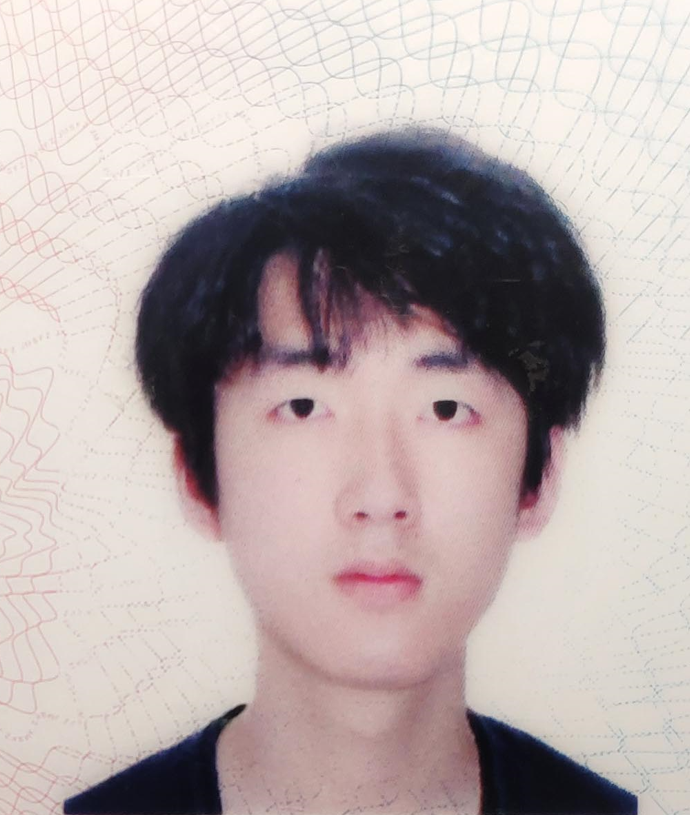
\includegraphics[height=8\baselineskip]{head.png}
% \end{minipage}

\basicInfo{
  \email{vanot313@gmail.com} \textperiodcentered\ 
  \phone{199-6730-0606} \textperiodcentered\ 
  \github[vanot313]{https://github.com/vanot313}}
 
\section{\faGraduationCap\  教育背景}
\datedsubsection{\textbf{浙江工业大学}, 杭州}{2018 年 9 月 -- 至今}
\datedsubsection{\textit{在读本科学士}\ 软件工程, 预计 2022 年 6 月毕业}{GPA 3.5(TOP 30\%)}

\section{\faUsers\ 项目经历}
\datedsubsection{\textbf{第十二届中国大学生服务外包创新创业大赛}}{2021 年 1 月 -- 2021 年 5 月}
\role{https://github.com/vanot313/project-data\_asset\_valuation-BC}{团队项目,担任队长}
\begin{onehalfspacing}
Flask 后端应用
\begin{itemize}
  \item 完成 flask 应用的 MVC 框架设计与简单的权限验证安全实现
  \item 采用 mysql 数据库,完成全部功能接口,数据接口编写
\end{itemize}
完整项目在服务端(ubuntu)的部署上线
\begin{itemize}
  \item 采用 docker 自动化部署方案,docker-compose 配置完成前后端应用的联合部署
  \item 采用 nginx 反向代理服务器,完成应用在服务端的集群部署
\end{itemize}
\end{onehalfspacing}

\datedsubsection{\textbf{网易 MiniGame 游戏大赛}}{2020 年 9 月 -- 2020 年 11 月}
\role{https://github.com/SharpLeaves/Core}{团队项目,担任程序兼策划}
\begin{onehalfspacing}
Unity 横板过关游戏
\begin{itemize}
  \item 负责游戏创意的策划,并完成游戏中关卡创意部分的实现(boss 的行为逻辑,与场景的交互逻辑)
  \item 完成游戏框架(状态机,人物碰撞模型与碰撞逻辑)编写,在 github 仓库中有对框架的介绍文档
\end{itemize}
\end{onehalfspacing}

\datedsubsection{\textbf{健康码管理系统}}{2020 年 5 月 -- 2020 年 7 月}
\role{https://github.com/vanot313/design-xhealthcode-BC}{个人项目}
\begin{onehalfspacing}
JavaWeb 全栈开发
\begin{itemize}
  \item 完成底层IoC框架(仿照Spring)以及完整后台系统框架与功能的编写
  \item 完成关系式数据库设计
\end{itemize}
\end{onehalfspacing}

% Reference Test
%\datedsubsection{\textbf{Paper Title\cite{zaharia2012resilient}}}{May. 2015}
%An xxx optimized for xxx\cite{verma2015large}
%\begin{itemize}
%  \item main contribution
%\end{itemize}

\section{\faCogs\ IT 技能}
% increase linespacing [parsep=0.5ex]
\begin{itemize}[parsep=0.5ex]
  \item 熟悉 Java、Python,了解 C++,熟悉数据结构与基本算法,有良好的编程风格
  \item 熟悉 Flask 框架、SSM、Springboot框架,了解 Vue 前端生态
  \item 熟悉 Docker,Nginx 等项目部署相关知识,了解 Linux 环境下操作
  \item 了解深度学习基本算法,LSTM长短时记忆神经网络
\end{itemize}

\section{\faHeartO\ 获奖情况}
\datedline{\textit{银奖}, ACM程序设计校迎新赛}{2018 年 11 月}
\datedline{\textit{三等}, 校奖学金}{2018 年 - 2019 年}
\datedline{\textit{二作}, 软件著作权}{2021 年}

\section{\faInfo\ 其他}
% increase linespacing [parsep=0.5ex]
\begin{itemize}[parsep=0.5ex]
  \item 参与学院学生会工作两年(负责学院创新分服务器以及微信公众号的开发与维护)
  \item 个人网站: http://vanot313.top
  \item 语言: 英语 - 熟练(CET 6)
\end{itemize}

%% Reference
%\newpage
%\bibliographystyle{IEEETran}
%\bibliography{mycite}
\end{document}
